\chapter{Development Process}
\label{chap:devProcess}

\begin{epigraphs}
\qitem{\textquotedblleft Make software that you want to use and that you would want to use often. As long as you are making something that you want to use, then your heart will be in it.\textquotedblright}%
      {Cabel Sasser, Sink or Swim, SXSW 2006}.
\end{epigraphs}
This chapter gives a full fledged description of the common software engineering techniques used to outline the process of this application's development. Read through to understand each process up close.

\section {UML or Unified Modeling Language}
\label{sec:uml}
UML is a method for envisioning a product program utilizing various semantic representation of information via simplified drawings. The documentation has developed from the craft by Grady Booch, James Rumbaugh, Ivar Jacobson, and the Rational Software Corporation to be utilized for object-oriented design, yet it has since been reached out to cover a more extensive assortment of programming building ventures. Today, UML is acknowledged by the Object Management Group (OMG) as the standard for demonstrating programming advancement.

\subsection{Why do we need UMLs}
A complicated linked systems\textquoteright \ enterprise application with many collaborators will require a solid foundation of planning and clear, concise communication among team members as the project progresses.\par \medskip

Visualizing user interactions, processes, and the structure of the system you\textquoteright re trying to build will help save time down the line and make sure everyone on the team is on the same page.

\section{Use case diagram}
A \textquotedblleft Use case diagrams\textquotedblright is a dynamic or conduct chart in UML. \textquotedblleft Use case diagrams\textquotedblright display the usefulness of a framework utilizing on-screen characters and utilize cases. Utilize cases are an arrangement of activities, administrations, and capacities that the framework needs to perform. In this unique situation, a \textquotedblleft system\textquotedblright is something being created or worked, for example, a mobile application. The \textquotedblleft actors\textquotedblright are individuals or elements working under characterized parts inside the framework.

\subsection{Why do we need use case diagrams}
\textquotedblleft Use case diagrams\textquotedblright are significant for envisioning the utilitarian necessities of a framework that will convert into outline decisions and advancement needs.\par \smallskip
They additionally help recognize any interior or outer components that may impact the framework and ought to be thought about.\par \smallskip
They give a decent abnormal state investigation from outside the framework. \textquotedblleft Use case diagrams\textquotedblright determine how the framework communicates with performers without stressing over the subtle elements of how that usefulness is executed.

\section{ASET ALiAS Native Mobile Application - System Name}
The \textquotedblleft system\textquotedblright is presented with a rectangular container which comprises of all the use cases of the system being developed. All the actors or on-screen characters are placed outside this system of use cases.

\subsection{Actors}
\textquotedblleft Actors\textquotedblright or the onscreen characters are the users of the system. This shall not result in the designer naming the actors with a Proper Noun, rather naming them as a role of someone who shall interact with the system being developed.
\begin{enumerate}
    \item admin
    \item User (student or faculty)
    \item Speaker (github link?)
\end{enumerate}

\subsection{Relationships}
Different shapes and designs of lines are used to define a relation between two different elements of the system. For example, a simple line is used for depicting the relation amidst an onscreen character also known as \textquotedblleft actor\textquotedblright and a particular use case. 

\subsection{Use Cases}
\textquotedblleft Use cases\textquotedblright are the next essential part of this system represented with oval shaped containers. The developer needs this diagram to adequately outline the needs of the app. The designer of this system enlists all the functions the actors are ought to perform after development of this project. These functions are referred to as use cases only when they result in a user\textquoteright s desirable outcome. \smallskip

 Hence, \textquotedblleft logging-in\textquotedblright cannot be considered as a use case while \textquotedblleft making a purchase\textquotedblright is a definite use case.\par \medskip

The primary use case of this application being developed is timely and efficient notification procedure as such announcements and updates help the concerned actor or user to stay up-to-date with other users and hence, stay in connection to the organization without having to pay attention to irrelevant content. \par


\subsubsection{Actor admin is responsible for}
\begin{enumerate}
    \item Posting highlights and announcements on a timely basis
    \item Upload new documents to the file library or the online database. These files can include event posters, talk resources, etc.
    \item Upload event information regularly
    \item Provide personalizing options 
\end{enumerate}
\subsubsection{Actor user accounts for the following user cases}
\begin{enumerate}
    \item Know about the concerned club and its members
    \item Have a good point of contact for a specific problem
    \item Get more information regarding an event and its speaker
    \item Receive timely notifications and announcements of club
    \item Personalize app according to preference
    \begin{enumerate}
        \item Get notified for all discussion forums or threads
        \item Opt into real-time updates or notifications only for threads the actor or user has participated in
        \item Complete opt out of notifications
    \end{enumerate}
    \item Read social media data like tweets from Twitter
    \item Know about local community groups and stay connected with them
\end{enumerate} \bigskip

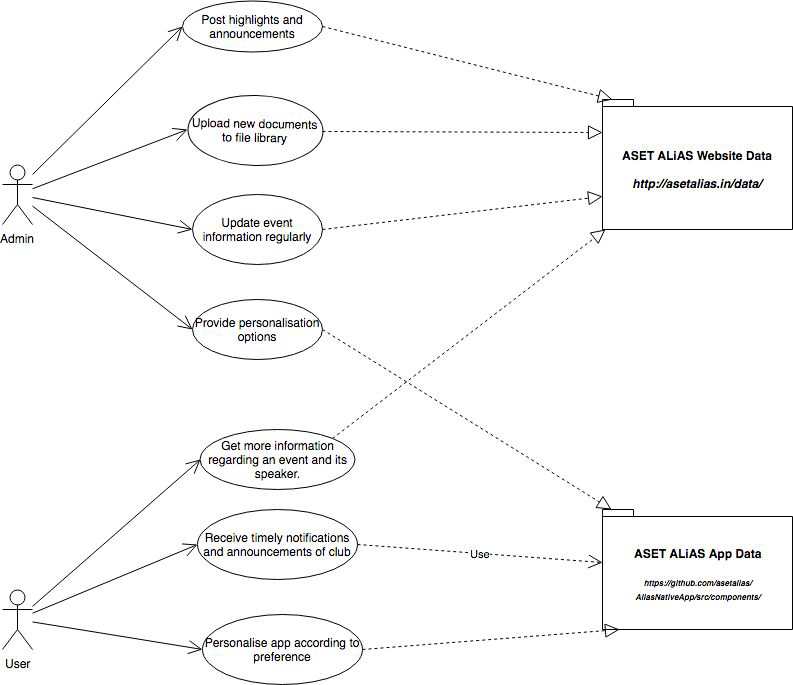
\includegraphics[width=150mm]{./alias-app-uml.png}\\